\section{Hardware}

\subsection{Board}

Board components are annotated in \Fref{fig:board}.  A detailed mechanical drawing describing the board dimensions and locations of key components is available on the \productWebPage{}.

\vskip 2em

\begin{figure}[H]
    \centering
    \begin{tikzpicture}[annotation/.style={circle, draw=black, fill=white, very thick, minimum size=7mm}]
        \node at (0,0) {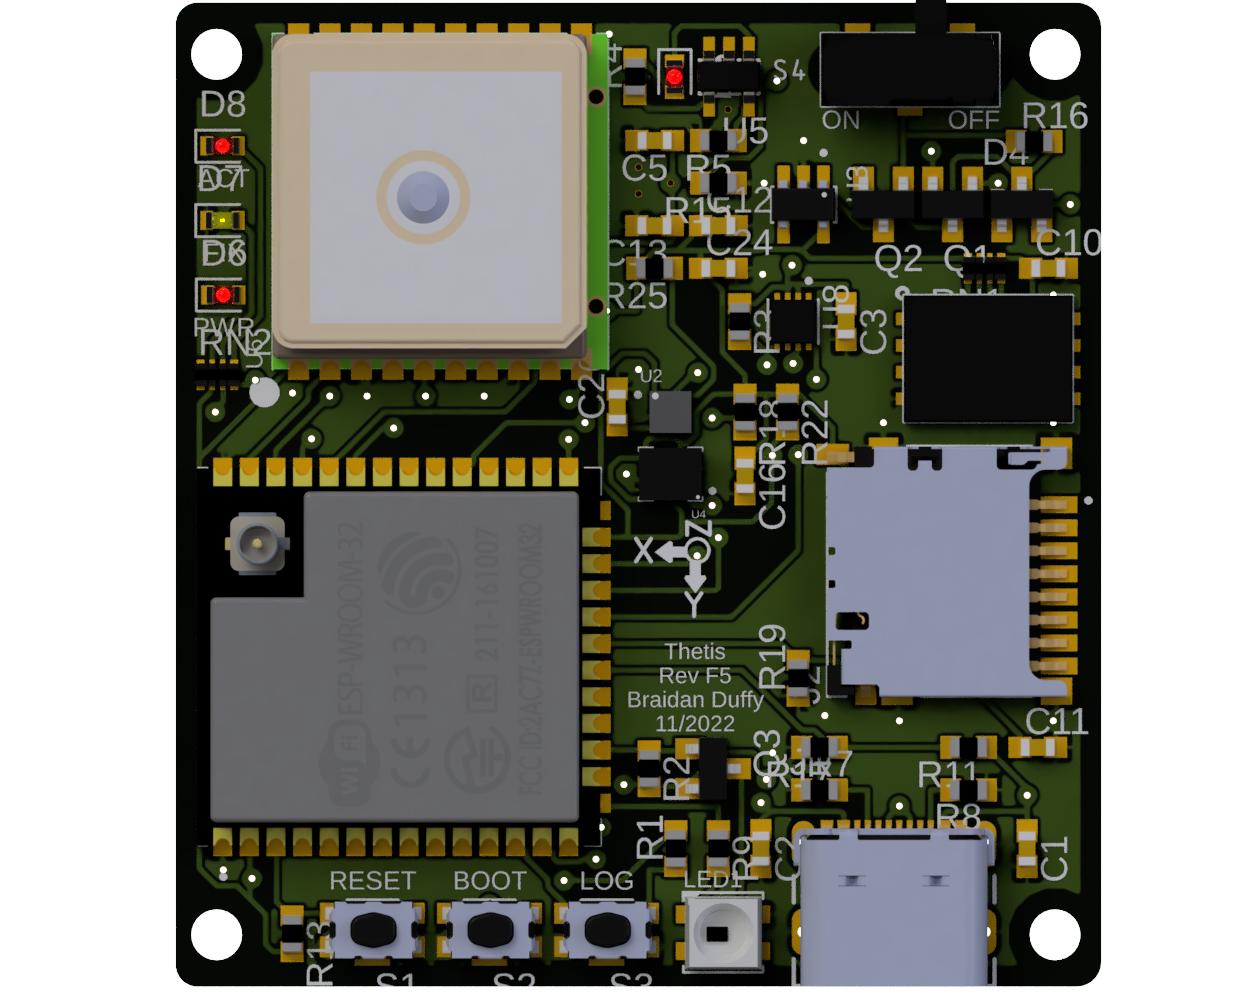
\includegraphics[width=0.95\textwidth]{Images/board.png}};
        \node[annotation] at (-6,-4) {\ref{itm:board1}};
        \node[annotation] at (-6.4,0) {\ref{itm:board2}};
        \node[annotation] at (-5.7,3.7) {\ref{itm:board3}};
        \node[annotation] at (-2.7,1.1) {\ref{itm:board4}};
        \node[annotation] at (4.8,1.8) {\ref{itm:board5}};
        \node[annotation] at (6.0,3.4) {\ref{itm:board6}};
        \node[annotation] at (7.2,3.4) {\ref{itm:board7}};
        \node[annotation] at (6.8,-1.9) {\ref{itm:board8}};
        \node[annotation] at (5.5,-4) {\ref{itm:board9}};
        \node[annotation] at (0.4,-0.8) {\ref{itm:board10}};
        \node[annotation] at (-3.4,-2.9) {\ref{itm:board11}};
    \end{tikzpicture}
    \caption{Board}
    \label{fig:board}
\end{figure}

\vskip 1em

\begin{enumerate}
    \item \label{itm:board1} Power button
    \item \label{itm:board2} \acs{USB}-C connector
    \item \label{itm:board3} \acs{LED}
    \item \label{itm:board4} Serial header
    \item \label{itm:board5} High-g accelerometer
    \item \label{itm:board6} Inertial sensor (gyroscope and accelerometer)
    \item \label{itm:board7} Magnetometer
    \item \label{itm:board8} Wireless antennae
    \item \label{itm:board9} U.FL connector for external wireless antennae
    \item \label{itm:board10} \acs{microSD} socket
    \item \label{itm:board11} Battery connector
\end{enumerate}

\clearpage

\subsubsection{Serial header}

\newcommand{\partNumber}[1] {\enquote{\href{https://www.samtec.com/products/#1}{#1}}}

The serial header pinout is annotated in \fref{fig:serialHeaderPinout}.  The connector part number is \partNumber{CLP-105-02-L-D}.  The recommend mating connector part number is \partNumber{FTS-105-03-F-DV}.

% import numpy

% width = 1.3
% height = 1.5
% pin = 1

% for y in numpy.linspace(height, -height, 5):
%     for x in numpy.linspace(-width, width, 2):
%         print("        \\node[annotation] at (" + "{:.2f}".format(x) + "," + "{:.2f}".format(y) + ") {" + str(pin) + "};")
%         pin += 1

\begin{figure}[H]
    \centering
    \begin{tikzpicture}[annotation/.style={draw=black, fill=white, very thick, minimum size=6mm}]
        \node at (0,0) {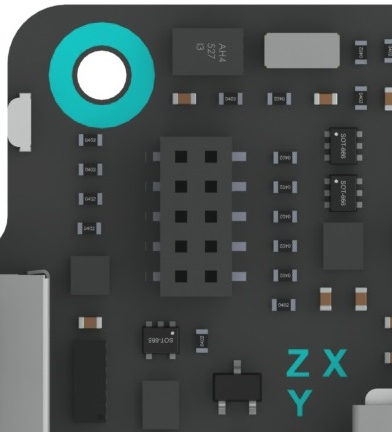
\includegraphics[width=0.5\textwidth]{Images/serialHeader.png}};
        \node[annotation] at (-1.30,1.50) {1};
        \node[annotation] at (-1.30,0.75) {2}; 
        \node[annotation] at (-1.30,0.00) {3}; 
        \node[annotation] at (-1.30,-0.75) {4};
        \node[annotation] at (-1.30,-1.50) {5};
        \node[annotation] at (1.30,1.50) {6};  
        \node[annotation] at (1.30,0.75) {7};  
        \node[annotation] at (1.30,0.00) {8};  
        \node[annotation] at (1.30,-0.75) {9}; 
        \node[annotation] at (1.30,-1.50) {10};
    \end{tikzpicture}
    \caption{Serial header pinout}
    \label{fig:serialHeaderPinout}
\end{figure}

\customTable
{l l l}
{Pin & Name & Type}
{
    1 & 3.3V & Power\\
    2 & GND  & Power\\
    3 & VBAT  & Power\\
    4 & VBUS  & Power\\
    5 & Button  & Input\\
    6 & Serial override & Input\\
    7 & Serial \acs{RTS} & Output\\
    8 & Serial \acs{CTS} & Input\\
    9 & Serial \acs{RX} & Input\\
    10 & Serial \acs{TX} & Output\\
}
{Serial header pinout}
{tab:serialHeaderPinout}

\vskip 1em

\warning{Incorrect connections to the serial header may cause permanent damage.  This interface should only be used by an experienced engineer.}

\clearpage

\subsection{Housing}

The housing interfaces are annotated in \Fref{fig:housing}.  A detailed mechanical drawing describing the housing dimensions is available on the \productWebPage{}.

\vskip 2em

\begin{figure}[H]
    \centering
    \begin{tikzpicture}[annotation/.style={circle, draw=black, fill=white, very thick, minimum size=7mm}]
        \node at (0,0) {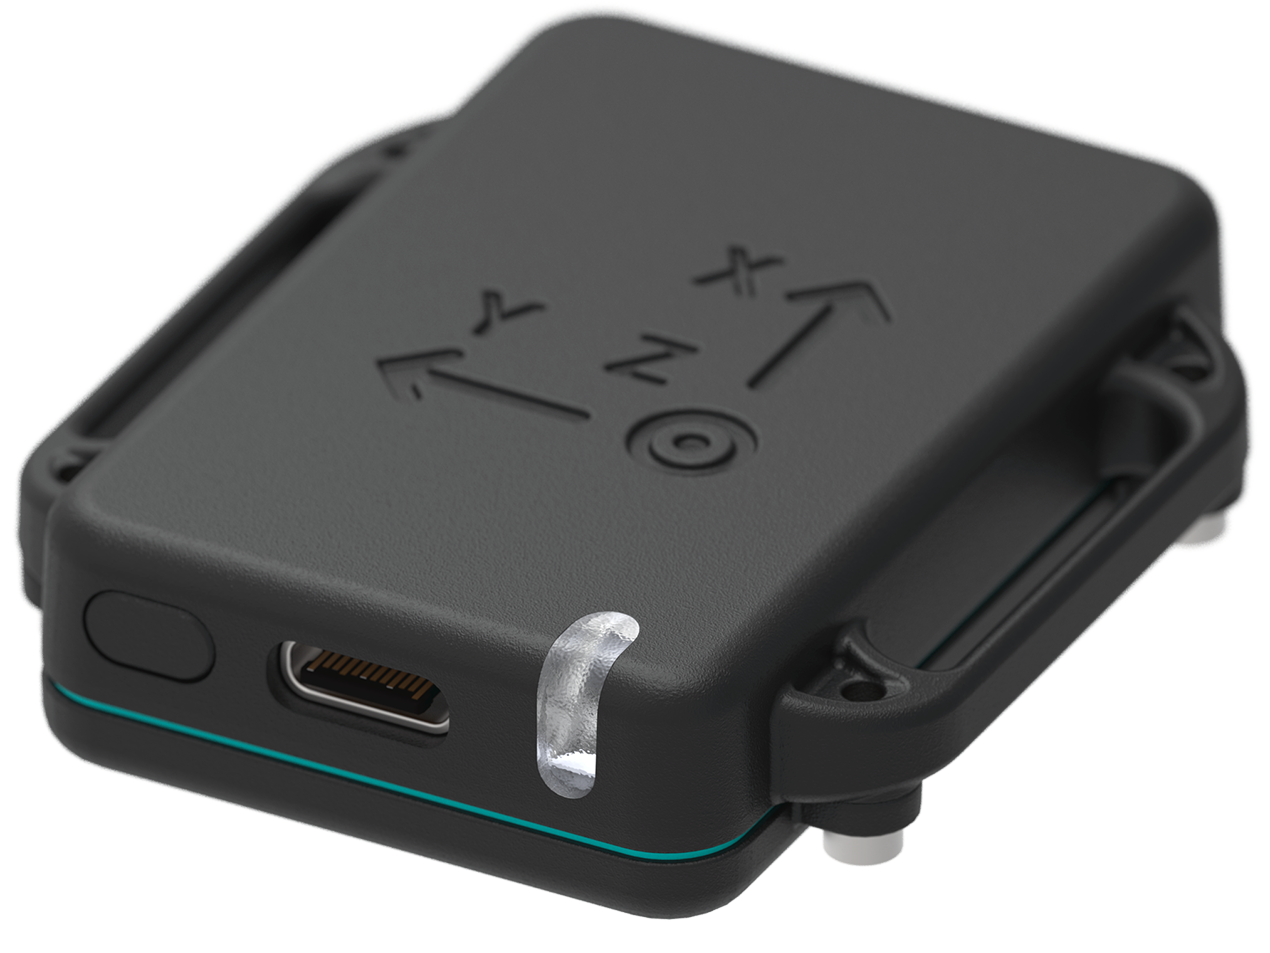
\includegraphics[width=0.8\textwidth]{Images/housing.png}};
        \node[annotation] at (-5.6,-2) {\ref{itm:housing1}};
        \node[annotation] at (-3.7,-2.55) {\ref{itm:housing2}};
        \node[annotation] at (-1.2,-3.2) {\ref{itm:housing3}};
    \end{tikzpicture}
    \caption{Housing}
    \label{fig:housing}
\end{figure}

\vskip 1em

\begin{enumerate}
    \item \label{itm:housing1} Power button
    \item \label{itm:housing2} \acs{USB}-C connector
    \item \label{itm:housing3} \acs{LED}
\end{enumerate}

\subsubsection{\acs{IP67} rating}

The \ac{IP67} rating is an international standard that describes the ability of the housing to protect against the ingress of solid particles and water.  The first digit, 6 indicates complete protection against dust and solid particles.  The second digit, 7 indicates protection from water for a maximum depth of 1 meter for up to 30 minutes.

In practical terms, this means that the housing can be used outdoors in all weather conditions and that it will survive accidental or temporary submersion in water.  The housing should \underline{not} be used in underwater applications.

\clearpage
